%!TEX root = *.tex
%%%%%%%%%%%%%%%%%%
% カウンタのリセット
\setcounter{figure}{0}
% 問題文
電場の中に置かれた正電荷を,電場から受ける力の向きに少しずつ移動させると,1本の線が得られる.
この線に沿って正電荷の移動の向きに矢印をつけたものを電気力線という.
電場の強さが$E$のところでは,電場に垂直な単位面積あたり$E$本の割合で電気力線を描く.
すなわち,電気力線は電場の様子を図で表現したものといえる.
この電場の中に導体をおくと静電誘導が起こるが,その後十分に時間が経ち,電流が流れていない状態になると,以下のことが成り立つ.
\begin{enumerate}[(\ajroman{\arabic{enumi}})]
  \setlength{\leftskip}{0zw}
  \setlength{\itemindent}{1zw}\setlength{\labelsep}{1zw}
  \setlength{\labelwidth}{1zw}
  \item 導体内部の電場は0となり,導体全体は等電位になる.
  \item 電気力線は,導体表面に垂直に出入りする.
  \item 電荷は導体内部には現れず,その表面だけに分布する.
\end{enumerate}


{
\begin{wrapfigure}{r}{6zw}
  \vspace{-\intextsep}
  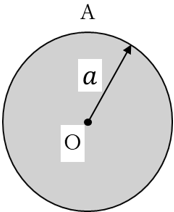
\includegraphics[width=6zw]{../graphs/open_19_8_2-1.png}
  \caption{}
\end{wrapfigure}



また,電荷分布と電気力線の関係として

\hang{「}
任意の閉じた曲面(閉曲面)の内部から外部に出る向きを正として,電気力線の本数は閉曲面内部の電荷の総和を$q$とするとき,$4\pi kq$本である.」

\noindent
が成り立つ.これはガウスの法則と呼ばれ,$k$はクーロンの法則の比例定数である.

以上述べてきたことをもとに以下の設問に答えよ.
\par}

\begin{enumerate}[\ajRoman{\arabic{enumi}}]
  \setlength{\leftskip}{-1zw}
  \setlength{\itemindent}{1zw}\setlength{\labelsep}{0.5zw}
  \setlength{\labelwidth}{1zw}\setlength{\leftmargin}{1zw}
  \setlength{\itemsep}{0.5\baselineskip}
  \item 図1のような半径$a$の導体球Aの表面に,正の電荷$Q$が一様に分布している場合を考える.
  \begin{enumerate}[(1)]
    \setlength{\leftskip}{-2zw}
    \setlength{\itemindent}{1zw}\setlength{\labelsep}{1zw}
    \setlength{\labelwidth}{1zw}
    \item 導体球Aの中心Oからの距離$r$の位置における電場の強さ$E(r)$を,$r>a,\,r<a$のそれぞれに対して求めよ.
    \item 導体球Aの中心Oからの距離$r$の位置における電位$\phi (r)$を,$r$の関数として求めよ.また,その様子を縦軸に$\phi$,横軸に$r$をとってグラフに描け.ただし,電位$\phi$の基準の位置を無限遠にとること.
    \item 導体球Aと無限遠は1つのコンデンサーを形成していると考えることができる.前問(2)の結果から,このコンデンサーの電気容量$C_A$を求めよ.
  \end{enumerate}
  \item 次に,内半径$b\,(>a)$,外半径$b+\delta$の薄い中空導体球Bの中に,半径$a$の導体球Aをその中心OがBの中心と一致するように配置する.以下の設問においても電荷分布の点Oに関する球対称性は保たれているものとする.
  \begin{enumerate}[(1)]
    \setlength{\leftskip}{-2zw}
    \setlength{\itemindent}{1zw}\setlength{\labelsep}{1zw}
    \setlength{\labelwidth}{1zw}
    \item 図2のようにAに正の電荷$Q$を与え,Bを十分遠方で接地(アース)する.このとき,AB間の電位差$V_{\rm AB}$を求めよ.また,この系をコンデンサーと考えたときの電気容量$C_1$を求めよ.
    \item 次に,図3のように,Aに被覆された導線をつなぎ,Bにあけた小穴を通してBの外側の十分遠方まで導線を伸ばしてAを接地し,Bの正の電荷$Q$を与える.この系のコンデンサーとしての電気容量$C_2$およびAB間の電位差$V^\prime_{\rm AB}$を求めよ.このとき,導線は十分に細いので,小穴部分の導線表面に分布する電荷は無視でき,また被覆物の影響も無視できるものとしてよい.
  \end{enumerate}
\end{enumerate}

\begin{figure}[H]
  \centering
  \begin{minipage}{.3\columnwidth}
    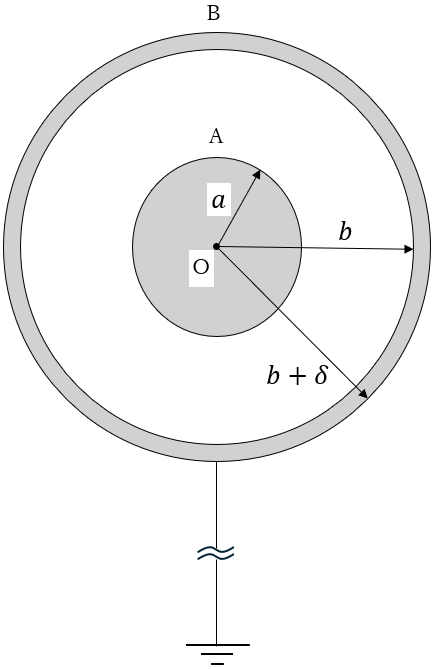
\includegraphics[width=\columnwidth]{../graphs/open_19_8_2-2.png}
    \caption{}
  \end{minipage}
  \hspace{.1\columnwidth}
  \begin{minipage}{.3\columnwidth}
    \centering
    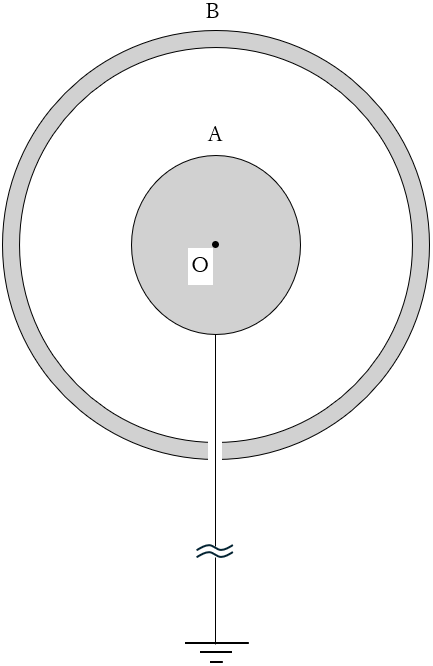
\includegraphics[width=\columnwidth]{../graphs/open_19_8_2-3.png}
    \caption{} 
  \end{minipage}
\end{figure}



%%%%%%%%%%%%%%%%%%